% Instructions to modify this document:
% * Remember to ALWAYS execute "git pull" BEFORE any commit you make!
% * Use the \ToDo{...} command to remark tasks which still need to be done. Add your name in the comment.
% * Use the \input{file.tex} command to split the document into several parts
% * Do not change the current LaTeX style to yours. The style and format should be homogeneous along sections.

% To graphviz to create diagrams with a textual description (.dot files) and then
% convert them to PDF.
% The .dot files are in the resources/ folder.

\documentclass[a4paper,12pt]{article}

\usepackage[utf8]{inputenc}
\usepackage{amsmath,graphicx}
\usepackage{bm}
\usepackage{amssymb}
\usepackage{algorithm}
\usepackage{algpseudocode}
\usepackage{subfigure}
\usepackage{ifpdf}
\usepackage{url}
\usepackage{color}
\usepackage[hidelinks]{hyperref}
\usepackage{multirow}
\usepackage{datetime}
\usepackage{comment}
\usepackage{float} % To put figures in their exact place with \begin{figure}[H]
\usepackage{longtable}
\usepackage{tabularx}
\usepackage{listings}
\usepackage{xcolor}
\usepackage[most]{tcolorbox}
\usepackage{parskip} % Avoid automatic indentation of every paragraph

\newcolumntype{L}[1]{>{\raggedright\arraybackslash}p{#1}}
\newcolumntype{C}[1]{>{\centering\arraybackslash}p{#1}}
\newcolumntype{R}[1]{>{\raggedleft\arraybackslash}p{#1}}


% Definitions and commands
\def \np{\vskip 0.25 cm}
\def \ap{\vskip 0.15 cm}

% JSON listing (see 
%  http://tex.stackexchange.com/questions/83085/how-to-improve-listings-display 
% -of- json-files)
\colorlet{punct}{red!60!black}
\definecolor{background}{HTML}{EEEEEE}
\definecolor{delim}{RGB}{20,105,176}
\colorlet{numb}{magenta!60!black}

\lstdefinelanguage{json}{
    basicstyle=\footnotesize\ttfamily,
    numbers=left,
    numberstyle=\scriptsize,
    stepnumber=1,
    numbersep=8pt,
    showstringspaces=false,
    breaklines=true,
    frame=lines,
    backgroundcolor=\color{background},
    literate=
     *{0}{{{\color{numb}0}}}{1}
      {1}{{{\color{numb}1}}}{1}
      {2}{{{\color{numb}2}}}{1}
      {3}{{{\color{numb}3}}}{1}
      {4}{{{\color{numb}4}}}{1}
      {5}{{{\color{numb}5}}}{1}
      {6}{{{\color{numb}6}}}{1}
      {7}{{{\color{numb}7}}}{1}
      {8}{{{\color{numb}8}}}{1}
      {9}{{{\color{numb}9}}}{1}
      {:}{{{\color{punct}{:}}}}{1}
      {,}{{{\color{punct}{,}}}}{1}
      {\{}{{{\color{delim}{\{}}}}{1}
      {\}}{{{\color{delim}{\}}}}}{1}
      {[}{{{\color{delim}{[}}}}{1}
      {]}{{{\color{delim}{]}}}}{1},
}

\lstset{language=Bash, basicstyle=\color{gray}}

\newcommand{\ToDo}[1]{\textcolor{magenta}{\textbf{[ToDo]} \textbf{#1}}}
\newcommand{\miguel}[1]{\textcolor{magenta}{\textbf{[Miguel]} \textbf{#1}}}


\begin{document}


\begin{titlepage}

\begin{center}
\vspace*{-1in}

\vspace*{0.6in}
\begin{Large}
\textbf{The IPOL Demo System 2.0 \\Technical documentation} \\
\end{Large}

\vspace*{0.6in}

\small{Compiled on \today\ at \currenttime}

\vspace*{0.6in}
\rule{80mm}{0.1mm}\\
\vspace*{0.1in}
\end{center}

\end{titlepage}

This document contains technical documentation for the IPOL Demo System 2.0. Specifically, the architecture of the service-oriented platform, its modules, and the real-time template generation of demos from their textual description.
\vspace*{0.6in}


\textbf{See the AUTHORS file at the project's root to see the list of authors}

%\maketitle
\newpage

\tableofcontents
\newpage
\listoffigures
\newpage

% Introduction
\section{Introduction}
\ToDo{Incomplete section!}

The system is built as a service-oriented architecture \cite{neuman2015building}.
The functionality is decomposed into a set of independent, self-contained microservice modules which communicate with each other via an API.

By splitting the monolithic application into smaller modules and decoupling interdependencies (between apps, dev teams, technologies, environments, and tooling), the system gains in terms of scalability, parallel development, easier debugging, and complexity isolation.

\begin{figure}[!ht]
\centering
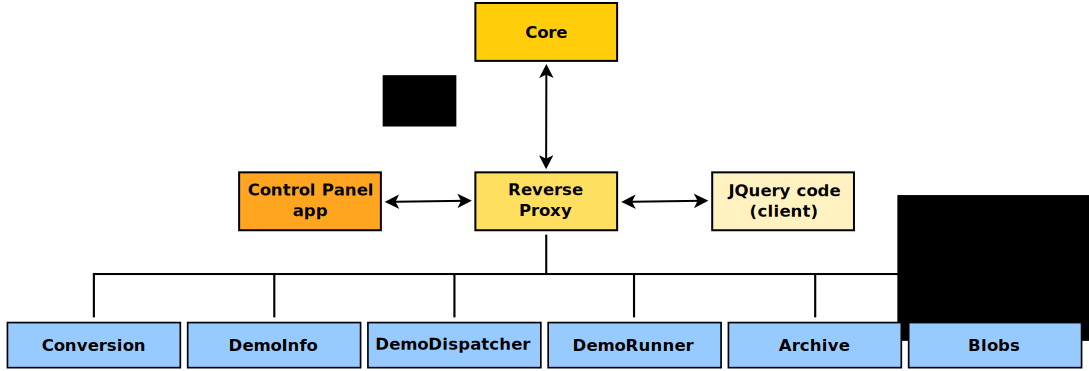
\includegraphics[width=0.8\linewidth]{architecture/images/architecture.pdf}
\caption{Modular system architecture.} 
\label{fig:architecture}
\end{figure}


% Project management and development methodology
% Project management and development methodology

\section{Development Methodology and Project Management}
The current IPOL project tries to follow the best practices in software engineering. Specifically, for this kind of project we found that Continuous Integration was a good choice in order to achieve fast delivery of results and ensuring quality. Continuous Integration is a methodology for software development proposed by Martin Fowler~\cite{fowler2006continuous} which consists on making automatic integrations of each increment achieved in a project as often as possible in order to detect failures as soon as possible. This integration includes the compilation and software testing of the entire project.

It is a set of policies that, together with continuous deployment, ensures that the code can be put to work quickly. It involves automatic testing in both integration and production environments. In this sense, each contribution in the IPOL system is quickly submitted and several automatic test are performed. If any of these tests fail the system sends an email indicating the causes.
%
Another advice of Continuous Integration is minimal branching. We use two. On one hand, master is the default branch and where all the contributions are committed. It is used for the development, testing and this continuous integration; on the other hand, the prod branch is used only in the production servers. It is merged with master regularly.
%
We use two different environments: integration and production. The integration server is where the master branch is pulled after each commit. The prod branch is used for the production servers and the code in this branch is assumed to be stable. However, the code in the integration server is also assumed to be stable and theoretically the code in the master branch could be promoted to production at any time once it has been deployed to the integration server and checked that is is fully functional and without errors. 

Quality is perhaps the most important requirement in the software guidelines of the IPOL development team. The code of the modules must be readable and the use of reusable solution is advised~\cite{GoF}. The modules must be simple, well tested and documented, with loose interface coupling, and with proper error logging. Note that it is not possible to ensure that any part of the IPOL will not fail, but in case of a failure we need to limit the propagation of the problem through the system and to end up with diagnostic information which allows to determine the causes afterwards.
%
Refactoring~\cite{fowler1999refactoring} is performed regularly and documentation is as important as the source code. In fact, any discrepancy between the source code and the documentation is considered as a bug.

Another tool used by the team is Trello. It allows to track the tasks of the project accoding to their current state (not assigned, assigned but not stated, assigned and in development, and finished). When a task arrives to the ``Finished" step, it is reviewed by the Project Director and archived (task totally finished) or moved back to development if more work is needed.

\begin{comment}
[ToDo]: move this to Sysadmin doc
The {\tt prod} branch was created with:
\begin{verbatim}
git checkout -b prod
git push --set-upstream origin prod
\end{verbatim}

The .git/config ends up as:

\begin{verbatim}
[core]
	repositoryformatversion = 0
	filemode = true
	bare = false
	logallrefupdates = true
[remote "origin"]
	url = git@github.com:mcolom/ipolDevel.git
	fetch = +refs/heads/*:refs/remotes/origin/*
[branch "master"]
	remote = origin
	merge = refs/heads/master
[branch "prod"]
	remote = origin
	merge = refs/heads/prod
\end{verbatim}

To merge {\tt prod} with {\tt master:}
\begin{verbatim}
git checkout prod
git merge master
git push
git checkout master
\end{verbatim}
\end{comment}


% Nginx as a reverse proxy
% Nginx as a reverse proxy

\section{Nginx as a reverse proxy}
\label{sec:reverse_proxy}
The IPOL project uses Nginx as a reverse proxy in order to redirect internet requests to the servers in the 
internal network. When Nginx receives a request, it decides which module it hast to send and so which machine that module is, 
then fetches the response, and sends it back to the client. With Nginx we implement private demos, microservise architecture 
patter and serve static files used by the clients.

\subsection{Static files}
The control panel as a Django web application needs to be compiled everytime the files change, so in order to serve the 
application Django offers a cli tool to collect all static files. Nginx serves all the static files used by the application and exposes them 
under a public route.

\subsection{API routing}
Nginx is also used to redirect incoming requests to the corresponding port and direction inside the machine where the module is 
running. Each modules has an internal file (sites-available) that decides where to route the request and deliver it to the desired endpoint.

\subsection{Private demos}
The IPOL system provides private demos that requires authentication by username and password. The ID of these demos begin with 
33333001. In this sense, Nginx can detect when a private demo is requested and it can forbid the access if the authentication fails.

% The Core module
\section{The Core module}
The Core is the centralized controller of the whole IPOL demo system. It controls the execution of the experiments and delegates tasks such as data pre-processing (Conversion module), execution dispatching (Dispatcher module), algorithm execution (DemoRunner module), archiving experiments (Archive module), or retrieving demo metadata, among others. It also sends email notifications when failures are detected during the execution of a demo, bad constructed DDLs or any other problem that needs to be notified to the user, the technical staff, or the IPOL editors.

When an execution is requested, it first obtains its textual description (its DDL) from the DemoInfo module. Then, it asks for the workload of the different DemoRunners and gives this information to the Dispatcher module in order to pick the best DemoRunner according to the Dispatcher's policy. The next step is to ensure that the source codes are compiled and updated in the corresponding DemoRunner. If the demo uses a DemoExtras file it is updated with its last version.

For the execution, the Core creates a run folder, copies the input data, and delegates any eventual pre-processing to the Conversion module. The run folder is identified by an unique key and it is created inside a folder which can be accessed by any machine of the IPOL's architecture. Therefore, all the DemoRunner machines can access the shared folder where the executions are performed. The DemoExtras are common files that are also visible and centralized.

Once the execution folder is ready, the corresponding DemoRunner runs the algorithm with the parameters and inputs set by the user. The Core waits until the execution has finished or after a timeout. Finally, the Core asks the system to store the experiment if the input data came from original data (uploaded by the user without private mode) or if the DDL specified to save all the executed experiments.

In case of any fatal failure (say, a conversion if needed but forbidden in the DDL, or the program of the article crashed), the Core terminates the execution and stores the errors in its log file. Eventually, it will send warning emails to the technical staff of IPOL (internal error) or to the demo editors.

Note that the Core does not need to know to which module it needs to delegate any operations, but instead simply requests the services using the IPOL API (see Sec. \ref{sec:reverse_proxy})

\subsection{DemoExtras}
\label{sec:demoextras} 
For the execution of some demos it is necessary some support code or data, which we refer to as \emph{DemoExtras}. This is not part of the peer-reviewed or published material, and it is only used by the demo.

The support files are stored in a package (say, .tar.gz, .zip, .tar, ...) in the DemoInfo module. Also, a copy of this compressed file is stored in the ``dl\_extras'' folder in the ``shared\_folder'' for comparison reasons. \ToDo{This mechanism should be explained in the demoInfo module section of the doc.}

The first time a demo is executed, the demos extras are decompressed in the ``DemoExtras'' folder in the ``shared\_folder''. At each execution the Core checks the date and the size of the compressed file in the ``shared\_folder'' with the one stored in demoInfo. \ToDo{This mechanism should be explained in the demoInfo module section of the doc. A diagram would be useful.}

The possible results from the check are:
\begin{itemize}
    \item \textbf{Date and size match}: nothing is done
    \item \textbf{Date or size do not match}: the DemoExtras are downloaded again
    \item \textbf{DemoExtras deleted in demoInfo}: all DemoExtras files related to that demo are deleted in the ``shared\_folder''
\end{itemize}

\subsubsection{Serving static content}
The {\tt html} directory of the demoExtras is served staticly by the system to allow the web interface access this data. It can be useful to show extra graphics or videos, or to allow the download of datasets in some especial demos.

For example, if in the demoExtras package of demo \#125 it exists a file ``image.png", it will be served from \url{http://ipolcore.ipol.im/demo/clientApp/static/125/image.png}


\subsection{Editor-controlled demo failures}
The Editor has the possibility to detect that some conditions are not met and notify the system that the execution of the demo failed, even if the program did not crash or the running script exited with a sucessful exit code. Indeed, a demoExtras script in the demo could check, for example, if the aspect ratio of the image is what the algorithm excepts, and prevent the actual execution.

The mechanism is simple: the editors can write a "demo\_failure.txt" file and stop the execution with an exit
code 0. The Core interprets the presence of this file as the demo itself signalling a problem.

For example, this code is used in one of the demos:
\paragraph{Example}:\\
\begin{verbatim}
imageSize=$(identify -format '%w+%h' input_0.png)
maskSize=$(identify -format '%w+%h' mask.png)

if [ $imageSize != $maskSize ]
then
  echo "Input error: input and mask have different sizes." >> demo_failure.txt
  exit 0
fi
\end{verbatim} 


\subsection{Interactive controls}
These are available in order to let the user draw on top of blobs. When adding an interactive control to the inputs of a demo, the core module will create files according to the data the interface sends before actual execution of the demo code. Here's a brief explanation for each kind of control.

\subsubsection{Mask control}
 For each input the core module will save an image with the name mask\_n.png, where 'n' is the number of the input with said control. This image comes from the client-side inside the run request.

\subsubsection{Dots and lines control}
The resulting text file will contain one line per coordinate on the image in a file in the execution folder, it will be named inpainting\_data\_n.txt where 'n' is the number of the input with said control.

Lines control will have the same result and processing by the core module as the dots control.

% The Blobs module
\section{The Blobs module}

\subsection{Introduction}
\label{sec:blobs_introduction}
The Blobs module introduction


% The Archive module
\section{The Archive module}

\subsection{Introduction}
\label{sec:archive_introduction}

%\paragraph{Introduction} \hspace{0pt} \\
The archive module is a standalone application destined to communicate with other modules using webservices. It is designed to implement a stable, simple and scalable system for archiving all experiments done with IPOL.

\paragraph{Technologies used} \hspace{0pt} \\
The archive module, written in Python, is using the cherrypy framework for webservices, the mako template library for webpage rendering, Python Image Library for thumbnails creations, and the python-magic library available on pip (not to be mistaken with python-magic5 which is the one available on ubuntu's default APT repositories). The module communicates using JSON, both in input and output. The database engine used is SQLite.

\subsection{Architecture}

\paragraph{Module composition} \hspace{0pt} \\
The module is composed of very few files, the code itself in ``module.py'', a cherrypy configuration file ``archive.conf'', two mako HTML templates, and a database. It will also need 4 directories, respectively for storing blobs, thumbnails, the database and logs.

\paragraph{Module architecture} \hspace{0pt} \\
The module is composed of a class, 'Archive', encapsulating the data needed to function. The services offered by the module are all methods of this class. The cherrypy framework provide the abstraction for making the methods available as webservices. \\
Upon starting the module, the cherrypy engine is launched, an object of the Archive class is created, and the cherrypy configuration is loaded from ``archive.conf''. If they don't exist, both the database and the directories needed for the storage of blobs, logs, the database and thumbnails will be created, provided that the user launching the module has the necessary rights. Otherwise, the module will not start. These directories are indicated in the cherrypy configuration for maximum configurability, if they are missing from it, the module will not start. \\
The webservices communicate with the server via arguments given through URL, as unicode strings directly passed to the methods. \\
The services all connect to the database in a thread-safe way, instanciating its own connection when called, commiting when done if there are modifications, or rollbacking, if there is an error, and closing the connection. \\
There is a logger initialised with the Archive object, writing errors in ``error.log'' in the logs directory given in the configuration file.

\subsection{Database design}

The database contains 3 tables : experiments, blobs, and correspondence.\\
Each experiments, and each blobs are defined individually, and linked to each-others in the correspondence table, assuring a many-to-many connection. It is worth noting that the database does not save duplicates of the same blob. \\

\ToDo{[Miguel] The right name for the ``correspondence" table is \emph{Junction table}. You can keep the name ``correspondence", but explain in the text that it is a junction table.}

\begin{tabular}{|l|c|r|}
  \hline
  experiments & blobs & correspondence \\
  \hline
  id & id & id \\
  id\_demo & hash & id\_experiment \\
  params & type & id\_blob \\
  timestamp & format & name \\
  \hline
\end{tabular} \\

\paragraph{Experiments table} \hspace{0pt} \\
The experiments table is defined as such : the id field, that stores the unique id of the experiment ; the id\_demo field, that stores the id of the IPOL demo used for the experiment ; the params field, which is a JSON string whose format varies from demo to demo ; and finally the timestamp field.

\paragraph{Blobs table} \hspace{0pt} \\
The blobs table is defined as such : the id field, that stores the unique id of the blob ; the hash field, that stores the hash of the blob computed with sha1, the type field, that stores the extension of the blob (e.g. ``jpeg'' or ``png''), and the format field, that stores the media format of the blob : it is a string, either ``audio'', ``video'' or ``image''. \\
The physical location of a blob is ``blob\_dir as defined in the configuration file'' + ``hash of the blob'' + ``.'' + ``type of the blob''.

\paragraph{Correspondence table} \hspace{0pt} \\
\ToDo{[Miguel] You can keep the name ``correspondence", but explain in the text that it is a junction table.}
The correspondence table is defined as such : the id field ; the id of the experiment and the id of the blob that is linked to said experiment, and the name field, which indicates the role of the blob in the experiment (example : ``input'' or ``denoised''). A foreign key constraint allowing cascade delete is put on the field id\_experiment, referencing the id of an entry in the experiment table, for automatic data deletion.

\subsection{Services}

\paragraph{Adding an experiment to the archive} \hspace{0pt} \\
Example :
\begin{verbatim}
http://<localhost>:<port>/add_exp_test?demo_id=42&blobs=
<json_blobs>&parameters=<json_parameters>
\end{verbatim}
The method ``add\_experiment'' takes in the entry of the id of the demo used ; a JSON string of the format : 

\begin{verbatim}
{
    url_blob : name,
    ...
}
\end{verbatim}

containing a description of each blob used by and produced by the experiment, with their temporary URLs and names ; and a JSON string describing the parameters of the demo used for the experiment. It will add an experiment to the database by creating a new entry in the experiment table. If the blobs used by and produced by the experiment aren't already in the database, it will copy them in the directory given in the configuration file, and create a thumbnail for the images. It will return a json string containing the status of the operation, OK if it succeeded, KO if there was an error and the operation wasn't performed, as such :

\begin{verbatim}
{
    status : OK/KO
}
\end{verbatim}

If status is KO, a log describing the error will be written.

\paragraph{Deleting an experiment from the archive} \hspace{0pt} \\
When removing an experiment from the database via the method ``delete\_experiment'', every blob linked to this experiment and only to this experiment is removed. After that, all the entries in the correspondence table referencing this experiment are removed automatically due to a foreign key constraint. It return a json response containing the status of the operation of the same format as the return of the method ``add\_experiment''. The method shouldn't be called anywhere else than through the user interface described later.

\paragraph{Deleting a blob from the archive} \hspace{0pt} \\
Due to a many-to-many link between blobs and experiments in the database, a blob has a lot of dependencies : it has of course the experiments using this blobs, but also the blobs linked to these experiments. For deletion of a blob from the archive, the precedent service is called on each experiment the blob is part of, assuring that no orphan data stay in the database (e.g. experiments linked to removed blobs or blobs linked to removed experiments). The method implementing this service is ``delete\_blob\_w\_deps''. It return a json response containing the status of the operation in the same format as the return of the method ``add\_experiment''. The method shouldn't be called anywhere else than through the user interface described later.

\paragraph{Getting data \ToDo{[Miguel] use a more specific word than ``data"} from an archive page} \hspace{0pt} \\
Example :
\begin{verbatim}
http://<localhost>:<port>/page?demo_id=42&page=3
\end{verbatim}
The method ``page'' returns a JSON response with, for a given page of a given demo, all the data of the experiments that should be displayed on this page. Twelve experiments are displayed by page. For rendering the archive page in the browser, the JSON response should be parsed and interpreted in a dedicated template furnished by the front-end of another module. The JSON response is formatted this way : 
\begin{verbatim}
{
    status :  OK/KO,
    experiments : [
        {
            date : timestamp_example, 
            files : [
                {
                    url : url_example,
                    id : id_example,
                    name : name_example,
                    url_thumb : url_thumbnail_example
                }
            ... ],
            id : id_example,
            parameters = {parameters_example...}
    ... ],
    id_demo : id_demo_example,
    nb_pages : nb_pages_example
}
\end{verbatim} 

\paragraph{Administrator interface for removing blobs/experiments} \hspace{0pt} \\
Example :
\begin{verbatim}
http://<localhost>:<port>/archive_admin?demo_id=42&page=3
\end{verbatim}
The only user interface furnished by the archive module is for removing blobs or experiment in a convenient manner. It uses the json response of the precedent service and renders the ``archive\_admin\_tmp.html'' template displaying a page of archives for given demo, allowing the deletion of both blobs and experiments by simply linking to two other services calling deletion methods and updating the template. In case of error, for example when invalid data is given through URL, ``error.html'' is rendered.

\paragraph{Shutdown} \hspace{0pt} \\
Example :
\begin{verbatim}
http://<localhost>:<port>/shutdown
\end{verbatim}
The method ``Shutdown'' shuts down the archive application when called. It returns a json response containing the status of the operation.

\paragraph{Other services} \hspace{0pt} \\
Other services features the method ``ping'', simply for checking if the module is up, and the method ``stats'', formatted this way :
\begin{verbatim}
{
    status : OK/KO,
    nb_experiments : x,
    nb_blobs : y
}
\end{verbatim}
Example :
\begin{verbatim}
http://<localhost>:<port>/ping
\end{verbatim}
Example :
\begin{verbatim}
http://<localhost>:<port>/stats
\end{verbatim}


% The Conversion module
\section{The Conversion module}
\label{sec:conversion}


\subsection{Introduction}
\label{sec:archive_introduction}

%\paragraph{Introduction} \hspace{0pt} \\
The conversion module is a standalone application dedicated to conversions of input files. 

\paragraph{Technologies} \hspace{0pt} \\
\begin{itemize}
\item Python (with packages available from PIP)
\item cherrypy (framework for webservices)
\item simplejson (required by cherrypy, JSON is the syntax to communicate with the module)
\item opencv-python (Python binding for the image processing library OpenCV)
\item libtiff (Python binding for the libtiff library, used to load and save tiff images)
\item numpy (a Python library for matrix calculation, used to modify image data)
\end{itemize}


\subsection{Image library}

Multiple libraries are available in Python to load and save images. IPOL has some requirements, in order of importance:

\begin{itemize}
\item open source,
\item available as a pip package,
\item support of data type other than integer 8 bits, especially in tiff (uint16, uint32, float16, float32),
\item exporting image data as a numpy matrix,
\item maturity and sustainability of the project,
\item intuitive API and good documentation,
\item fast.
\end{itemize}

\paragraph{OpenCV} \hspace{0pt} \\
Many libraries have been tested, the final choice has been OpenCV. OpenCV (Open Computer Vision) is a well known open source library in the domain of computer vision. It is a C++ program with a Python binding. After tests, it appears that loading and saving tiff files was not correct for uint32, float16 and float32 formats, reason why libtiff is used in IPOL for loading and saving tiff images. The documentation could be improved, the API is a bit conplex, but globally, OpenCV is efficient, with intesting algorithms (even they are not yet used by IPOL).

\paragraph{libtiff} \hspace{0pt} \\
Libtiff is a Python wrapper of the classical C libtiff library providind numpy.memmap view of tiff files. This library is more tested than OpenCV to load and save exotic TIFF formats, the numpy data can be converted to the OpenCV format.

\paragraph{pillow} \hspace{0pt} \\
Pillow is the most common Python library for images. It is well documented with a simple API, but, it does not support other formats than the common integer 8 bits.

\paragraph{ImageMagick} \hspace{0pt} \\
ImageMagick is a classical C library used with command line, and also available in with other languages. There are too many Python bindings, most are badly supported or discontinued. Wand is the most known library, but it is not yet available by pip. There are also problems in ImageMagick API to control the Tiff parameters for saving.

\paragraph{GDAL} \hspace{0pt} \\
GDAL (Geospatial Data Abstraction Library) is a C library dedicated to geospatial images, with a Python wrapper. It handles a vast list of specific formats, and among tham, have a decent tiff support. It is supposed to be available by pip, but installation does not work. It is possible to install python-gdal as a Debian package, but this produces insconsistency in Python packages when used in conjunction with pip, especially for numpy.

\paragraph{SimpleITK} \hspace{0pt} \\
ITK is a C++ library to process medical images. SimpleITK is a layer on ITK, supposed to simplify the API for script languages. The library is working well, available by pip, but the API is not stable enough to invest code on it.

\paragraph{pyPNG} \hspace{0pt} \\
PyPNG is a pure Python library, handling the PNG format. It could be very slow (40 times more than OpenCV on read for big images). 

\paragraph{imageio} \hspace{0pt} \\
Imageio is a Python library that provides an interface to read and write a wide range of image data for numpy. But it has no original code, it silently choses among plugins like Pillow, OpenCV or SimpleITK, according to the extension, but without access to all the options of the original library.

\paragraph{scikit-image} \hspace{0pt} \\
Scikit is a Python library for image processing, designed to interoperate with scipy and numpy. This solution maybe promoted to handle images other than integer 8 bits, but it uses OpenCV behind the API.





% The Demo Info module
\section{DemoInfo module}
This module store the textual description of the demo and allows to ask for specific sections of it. It also stores other demo-related information, as:
\begin{itemize}
\item Demo id
\item Abstract
\item Title 
\item Authors list
\item Authors email list
\item Article URL
\item State (inactive,preprint, published)
\item Demo editor
\item Demo editor email
\item Demo zip file containing demo DDL 
\item Demo DDL JSON
\end{itemize}

\subsection{DemoInfo module structure}
This Module is made of:
\begin{itemize}
  \item model.py where the db structure, the DAO (Data access object) classes and some helper classes (Demo, Author and Editor) are defined. It provides a layer of abstraction over the DB.
  \item demoinfo.py it's the module.
\end{itemize}

\subsection{The model (database) structure}
The model of this module id made of the following tables:

\begin{figure}[!ht]
    \centering
    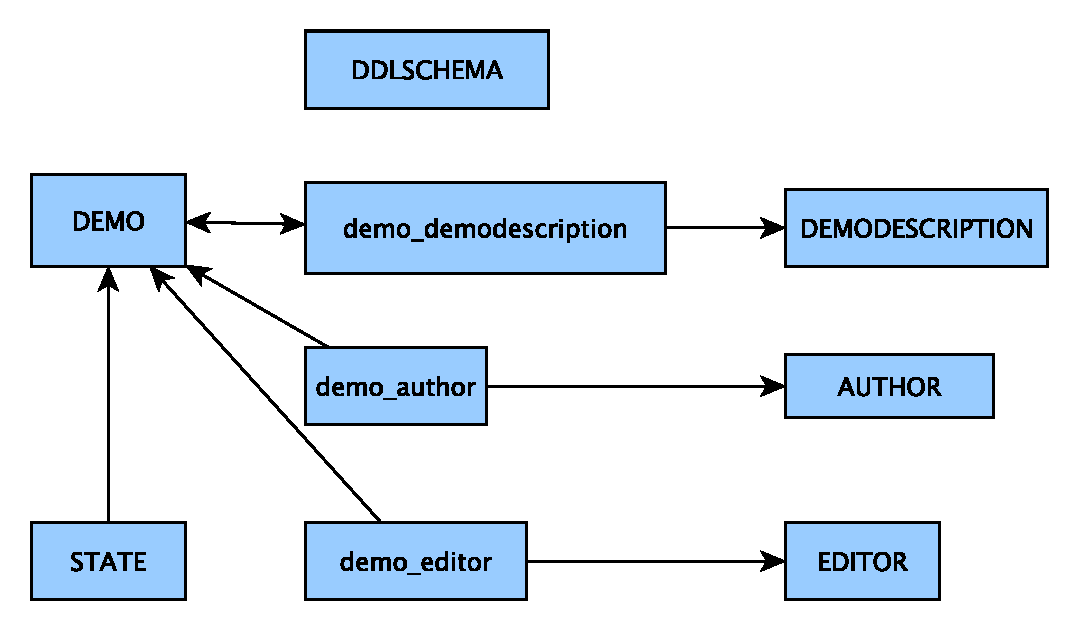
\includegraphics[width=0.8\linewidth]{demoinfo/images/demoinfo_model.pdf}
    \caption{Demoinfo database model.}
    \label{fig:demoinfo_model}
\end{figure}

Note that states is the table for the demo's state (published, preprint, \dots)
The Demodescription table is where the DDL of each demo is stored.
A demo may be created without a DDL (but you will need to provide one so you can run it)

\begin{itemize}
\item  demo\_list(self)
\item  demo\_list\_by\_demoeditorid(self,demoeditorid\_list)
\item  demo\_list\_pagination\_and\_filter(self,number\_elements\_page,page,qfilter=None)
\item  demo\_get\_authors\_list(self,demo\_id)
\item  demo\_get\_available\_authors\_list(self,demo\_id)
\item  demo\_get\_editors\_list(self,demo\_id)
\item  demo\_get\_available\_editors\_list(self,demo\_id)
\item  demo\_get\_demodescriptions\_list(self,demo\_id,returnjsons=None)
\item  read\_demo\_metainfo(self, demoid)
\item  read\_demo\_metainfo\_by\_editordemoid(self, editordemoid)
\item  add\_demo(self, editorsdemoid, title, abstract, zipURL, active, stateID, demodescriptionID=None, demodescriptionJson=None)

    Allows you to create a demo
    \begin{itemize}
        \item allow only post
        \item only creating the demo
        \item creating the demo and assigning an existing ddl (with id demodescriptionID) to it
        \item create the demo and create a ddl , with the json passed by param (demodescriptionJson)
    \end{itemize}

\item  delete\_demo(self,demo\_id,hard\_delete = False)
allow only post
\item  update\_demo(self,demo)
allow only post
\end{itemize}


AUTHOR

\begin{itemize}
\item  author\_list(self)
\item  author\_list\_pagination\_and\_filter(self,number\_elements\_page,page,qfilter=None)
\item  read\_author(self, authorid)
\item  author\_get\_demos\_list(self,author\_id)
\item  add\_author(self,name, mail)
allow only post
\item  add\_author\_to\_demo(self,demo\_id ,author\_id)
allow only post
\item  remove\_author\_from\_demo(self,demo\_id ,author\_id)
allow only post
\item  remove\_author(self,author\_id)
allow only post
\item  update\_author(self,author)
allow only post
\end{itemize}


EDITOR

\begin{itemize}
\item  editor\_list(self)
\item  editor\_list\_pagination\_and\_filter(self,number\_elements\_page,page,qfilter=None)
\item  editor\_get\_demos\_list(self,editor\_id)
\item  read\_editor(self, editorid)
\item  add\_editor(self,name, mail)
allow only post
\item  add\_editor\_to\_demo(self,demo\_id ,editor\_id)
allow only post
\item  remove\_editor\_from\_demo(self,demo\_id ,editor\_id)
allow only post
\item  remove\_editor(self,editor\_id)
allow only post
\item  update\_editor(self,editor)
allow only post
\end{itemize}

DDL

\begin{itemize}
\item  read\_demo\_description(self, demodescriptionID)
\item  read\_last\_demodescription\_from\_demo(self,demo\_id,returnjsons=None)
\item  add\_demodescription\_to\_demo(self,demo\_id, demodescription\_id)
allow only post
\item  add\_demo\_description(self,demoid=None,inproduction=None)
allow only post
\item  add\_demo\_description\_using\_param(self, demojson,inproduction = None)
\item  update\_demo\_description(self, demodescriptionID)
\end{itemize}

MISCELLANEA

\begin{itemize}
\item  index(self)
\item  ping(self)
\item  shutdown(self)
\item  stats(self)
\item  read\_states(self)
\end{itemize}


% The Demo Dispatcher module
\section{Dispatcher module}
\label{sec:Dispatcher}
In order to distribute the load in several machines, this module is responsible to assign a demorunner according to a policy and the given requirements. 
The creation of those policies is made by the Factory Method, allowing the implementation and assignment of new policies in an easy way.
Until now the implemented policies are:

\begin{itemize}
\item \textbf{Random Policy:} this policy assigns a random demorunner from the available demorunners list that matches the requirements 
\item \textbf{Sequential Policy:} this policy iterates from the available demorunners list that matches the requirements 
\item \textbf{Lowest Workload Policy:} this policy assigns the demorunner with the lowest workload from the available demorunners list that matches the requirements 
\end{itemize}


% The Demo Runner module
\section{DemoRunner module}
\label{sec:DemoRunner}
This module controls the execution of the IPOL demos. In order to achieve the Reproducible Research that the journal seeks, the DemoRunner must ensure that the users can reproduce exactly the results claimed by the authors of the paper. In this sense, each experiment is done with the last source codes provided by the authors.

Before each execution, the Core module prepares a run folder for the experiment with the input files converted according to the DDL specifications. We need several machines in order to execute several demos at the same time by sharing the load among them. This leads to a distributed system with several DemoRunners (see section~\ref{sec:Dispatcher}). Thanks to this, the Core can request to run the algorithms at the machine that best fits according to the load balancing policy set in the system. For this, DemoRunner is responsible of informing the Core about the load of the machine where it is running on. This allows to have several machines with different requirements for the demos (Matlab, specific libraries, among others)

The DemoRunner module executes the experiment to produce output files according to this workflow: (i) ensure the compilation, (ii) control and execute the experiments and, (iii) control exceptions and failures. 

\paragraph{Ensure compilation}
\noindent

This is an important step because this ensures that IPOL always uses the last version of the source codes provided by the authors. 

The first time that a demo is executed, the module downloads, extracts and compiles the source codes directly from an URL that must be given by the DDL. This URL is the link where the author's codes are stored. If this process is successful, the module moves the requested executables to its binaries directory and keeps them for the following executions.

Henceforth, DemoRunner will compare differences between the information from the HTTP header of the linked file with its local copy. If there have been any modifications in the size or the dates, the system will understand that new source codes are provided and it will download and compile them again. 

\paragraph{Control and execute the experiments}
\noindent

The second responsibility of the module is to control the execution.  It can execute directly the authors binaries or, for more complex process, supporting scripts provided by the demo editors related to a particular demo (see more about \textit{DemoExtras} in section~\ref{demoextras}). Besides, the demo editors can use some generic scripts in their \textit{DemoExtras} to represent their results such as draw 2D curves, draw histograms, counting lines, among others. These ones are provided by the IPOL System and they are stored at each DemoRunner module. We refer to these scripts as \textit{PythonTools}.

Before an experiment, the module receives all the information that it needs, such as the the ID of the demo, the execution key, a suggested time for stopping execution (avoiding experiments that take too much time), and the parameters set by the user in the web interface.

Normally, the results files are read by the web interface according to the information in the DDL. For instance, if a particular demo creates an output image with the name '\textit{output.png}' and the results section in the DDL sets that this image is the output, the web interface looks in the run folder of the experiment and uses it to create a link for the Image Gallery. This Image Gallery is a service for displaying results according to the DDLs.

Nevertheless, in other cases the process is not so simple and some additional mechanism is needed to show the results.  Let's suppose an optical flow demo. Usually, this type of demos uses a pair of consecutive images as input to calculate the displacement field between them. However, sometimes you can also include a ground truth that represents exactly the motion present between the inputs. This ground truth helps to measure how close is your solution respect to the best possible flow field using different error measures. For this, it is mandatory that the web interface distinguish between these two types of executions. 

Another example is a demo with a variable number of outputs. The web interface needs to know how many times it needs to repeat, but this information is only known after the execution. Thus, the demo editor can write this file and add a variable which will be used by the web interface to draw the repeat gallery.

In this sense, the DemoRunner module provides a mechanism for recovering the information about the results of an execution. The editor of a demo can store information from the execution in a text file (algo\_info.txt). The module reads this file to obtain the names of the variables and the values that it contains and gives it back. For instance, the demo can write the number of outputs generated in the file and the Core can return it to the web interface so it can be shown according to the DDL specifications.

\paragraph{Control exceptions and failures}
\noindent

The module takes care of stopping the demo execution if a problem appears such as not supported inputs for the demo, a bad implementation of the source codes or the demoextras, incorrect syntax in the run section at the DDL, among others. In these cases, DemoRunner notifies about the causes of the failure so the Core can take the best action. 

Another reason for stopping an execution occurs when a demo exceeds a reasonable running time, either because of a malfunctioning on the author's program that produces that it might never finish or simply because the execution time is too large for a demo. Related to this, the demo editors can include a maximum value (timeout) in their DDLs for the executions of their demos. Therefore, the Demorunner will stop the experiment if a timeout is reached and the algorithms have not finished. Otherwise, the module will assign its own security timeout and likewise, if the time set in the DDL is excessive or too short, the DemoRunner will modify this to a more reasonable value.


% The Access Control 
\section{Access control}
\label{sec:Access_control}
\subsection{Introduction}
To avoid the execution of exposed methods that allow the modification of the database (write and delete actions) by an unauthorized 
client, it has been created a wrapper that controls the access to these methods.

This wrapper compares the IP of the client that is calling the method with a list of authorized patterns. If the IP is authorized, 
the wrapper will automatically invoke the method requested by the client. Otherwise the request will be denied and the wrapper will 
respond with an Authentication Failed message.


\subsection{Authorized IPs File}
The file with the authorized IPs patterns is authorized\_pattern.conf, in the config\_common directory. This file consists
of a general section [Patterns], where all the permitted patterns are given with the following format: ``name=pattern''. Each pattern
allows the access of multiple IPs. 

The syntax for the pattern uses the asterisk to mean ``any''. For example: {\tt``local = 127.*.*.*''}

\subsection{Usage}
To add the authentication requisite to a method it is enough to add the {\tt@authenticate} decorator. It is important to add it 
below the {\tt@cherrypy.expose} decorator. Otherwise the method will not be longer exposed.


% Tools
\section{Tools}
This section describes the tools available for system administrators, developers, and editors to interact with the IPOL system. Some of their capabilities might clash with the Control Panel (for example, reading and modifying the DDL of the demos in the case of the DDL tool, Sec. \ref{sec:ddl_tool}), but they are useful to perform massive changes or to automatize tasks.


\subsection{DDL tool}
\label{sec:ddl_tool}
\ToDo{Document the DDL tool}


% Tests
\section{Tests}
\label{sec:Tests}
\subsection{Introduction}

The objective of the tests is to analyze automatically if the system fits the intended use. For that purpose the system is analized with two
types of tests, the first one are the Integration Tests in which individual software modules are combined and tested as a group, this implies from
the creation of a demo to its execution. The second one are the Unit Tests that are executed for each module and checks the response of all the
exposed methods.

Those tests are automatically executed in the integration and production enviroments every day by the crontab and every time a pull is made by 
the terminal.py script. If any of those test fail, an email is sent to all the emails listed in the /ci\_tests/send\_to.txt file.


\subsection{Integration Tests}

The integration tests are located in the /ci\_tests/system.py script and are responsible for testing all the IPOL modules and the interactions
between them. To accomplish that goal each test execute the full flow of the system, that goes from the creation of a demo, adding the DDL, blobs,
demoExtras, etc. to the execution of it.

Each test is independent from the others so the order in which it is executed is not important. To ensure that the state of the system has not been
altered by other test, the function setUp() is executed before every test. This function is responsible for cleaning the database from the 
remains of other tests.

\subsection{Unit Tests}

On each module there is a test.py script that executes all the unit test of the module. Each test check the correctness of every exposed method.

In the same way as the integration tests, each test can be executed in any order since the state of the system should not change after the execution
of the test.

\subsection{All.py}

This script is responsible for executing all the test, both the integration (system.py) and the unit test (test modules). To ensure
That several tests are not executed simultaneously, which could cause failures in the tests, a blocking system is implemented by the creation 
of the test.lock file, which if it exists implies that another instance of this script is running the tests.
If the script is blocked by this file it waits a random time between 5 and 10 seconds and check it again until it can run.


\subsection{Pull.sh}

This script is responsible for executing the git pull and call the all.py script to start all the tests. If any of the executed test fails an email
will be send to the email list reporting the failure.

This script is executed periodically every day at 10:00 am by the following instruction in the crontab: \begin{lstlisting}[language=Bash]
 0 10 * * * /home/ipol/ipolDevel/ci_tests/pull.sh
\end{lstlisting} in order to detect possible failures in the integration and production
enviroments, e.g. down modules, lack of disk memory, etc. Or every time a pull is made from the terminal.py script to check if the added cahnges do not
damage the system.


% Installation
\section{Installation of the project}
When new members arrive at the development team they need to set up their environment. This section lists the actions needed.

\paragraph{General} \hspace{0pt} \\
\begin{itemize}
 \item Install Debian Stable.
 \item Signup in Trello, Github, and Slack.
 \item Add the emails of the new members to the send\_to.txt file (in ipolDevel/ci\_tests/).
 \item Sign up in our Demo Editing group in Google Groups
 \item Create a new RSA key with {\tt ssh-keygen}
 \item Clone the repository from GitHub: {\tt git clone git@github.com:mcolom/ipolDevel.git}
 \item Download a good Python IDE. For example: Pycharm.
\end{itemize}

\paragraph{SSH} \hspace{0pt} \\
\begin{itemize}
 \item Add your public key to the authorized\_keys file in the servers.
 \item Optional: Install the SSH server in your machine and add your public key to your own authorized\_keys to start the modules with the IPOL Terminal.
\end{itemize}

\paragraph{Documentation} \hspace{0pt} \\
\begin{itemize}
 \item Download a \LaTeX editor. For example: Kile.
 \item To be able to compile the documentation install texlive-full.
  \begin{lstlisting}[language=Bash]
  ~/sudo apt-get texlive-full
  \end{lstlisting}
 \item Generate all the PDFs of the documentation.
\end{itemize}

\paragraph{Libraries} \hspace{0pt} \\
\begin{itemize}
 \item Install all the python libraries with the following command:
  \begin{lstlisting}[language=Bash]
  ~/pip install -r requirements.txt
  \end{lstlisting}
 \item Install all the libraries described in doc/system/ipol.pdf in the ``general\_notes'' section.
\end{itemize}

\paragraph{NGINX} \hspace{0pt} \\
\begin{itemize}
 \item Install nginx.
  \begin{lstlisting}[language=Bash]
  ~/sudo apt-get install nginx
  \end{lstlisting}
 \item Copy the config files that are in sysadmin/configs/nginx/default-local into the nginx folder /etc/nginx/sites-available/default and change the variable \$my\_user
\end{itemize}

\paragraph{Modules} \hspace{0pt} \\
\begin{itemize}
 \item Copy manually all the files that are not in the repository:
 
  \begin{itemize}
   \item ipol\_demo/modules/config\_common/authorized\_patterns.conf
   \item ipol\_demo/modules/config\_common/emails.conf
  \end{itemize}

 \item Copy from integration the DB and the staticData from the demoinfo and blobs modules.
 \item Update the XML files in config\_common
\end{itemize}

\paragraph{Control Panel} \hspace{0pt} \\
\begin{itemize}
 \item Add the hostname to the list ``local\_machines'' in the file ipol\_webapp/ipol\_webapp/ settings.py
 \item Follow the steps described in ipol\_webapp/docs
 \item Create a new superuser in the local Control Panel
  \begin{lstlisting}[language=Bash]
  ~/ipolDevel/ipol_webapp/python manage.py createsuperuser
  \end{lstlisting}
\end{itemize}


% User scripts
\section{User scripts}
The demo system provides some scripts common tasks, to free the demo editors to re-invent the wheel writing the same code multiple times.
In this section we document them briefly.

\subsection{draw2Dcurve.py}
A simple script utility to draw single and multiple 2D plots using matplotlib.


\subsection{Video editing tools}
This is for those authors who are unable to read a video file but instead they prefer to have the video as a bunch of frames.
Thus, the system will save the frames as {\tt input\_0/frame\_00000.png}, {\tt input\_0/frame\_00001.png}, {\tt input\_0/frame\_00002.png}, \dots
If there are several inputs, they will be {\tt input\_1}, {\tt input\_2}, etc.

The system offers some helpers you can call from your demoExtras:
\begin{itemize}
    \item {\tt website\_mp4.sh}: converts a video of any format to a (lossy compressed) MP4 video that can be show in the web interface. Only for visualization. You can later offer to download original data.
    \item {\tt frames\_to\_avi\_huff.sh}: reads the frames extracted from a video and creates a Huffman-encoded (lossless) AVI file.
    \item {\tt frames\_to\_mp4.sh}: reads the frames extracted from a video and creates a lossy MP4 file. Only for visualization.
    \item {\tt get\_video\_fps.py}: prints the video's frame's per second (FPS).
\end{itemize}

\subsection{ply2obj.py}
Converts a .ply mesh (Stanford) to a .obj mesh (wavefront).


% General notes
\section{General notes}
In this section we add general comments on the projects, parts which still neeed to be written or coded. In general, information which needs to be documented but has not still found its place in the document. It works as a reminder not to forget.

\begin{itemize}
    \item The magic module. We use PIP, not the python-magic package found in most distributions. \ToDo{Explain why}.

    \item Example of another demo system: \url{http://places.csail.mit.edu/demo.html}

    \item Integrate Openseedragon, \url{https://openseadragon.github.io/}

    \item Document the format of the demo package, with desc.jon, images/, extra/, etc

    \item Most of our modules name the files according to the hash sum of their contents. This file names are OK for internal use, but the users should obtain the files with the proper names. This can be achieved with the ``download" attribute in HTML5. All website interfaces should provide the corresponding human-readable name. For example:
        \begin{verbatim}
<a href="9021384984901238.png" download="denoised.png">
  Download the denoised image
</a>
        \end{verbatim}

    \item Look for potential race conditions everywhere in the code, specially at the modules. Use locks to prevent them.

    \item In general, check that no FK reference is missing at any of the database schemas of the modules, and that they're correct.
          Also, we need to check absolutely that all the CASCADE DELETE are correct!

    \item FYI: the package \emph{sqlitebrowser} seems to be a very good tool to browse and develop the SQLite schemas.

    \item Check that all modules return application/json and Content-Type: text/json;charset=utf-8

    \item A way to get images from the browser in a smartphone with HTML5: \url{http://don.github.io/html-cam/}
\end{itemize}



\subsection{To Do}
- Add statistics data collecting. Piwik can be used for this. Or Google Analytics, amongs others.


\bibliographystyle{plain}
\bibliography{biblio}

\end{document}
% End of document

